\subsubsection{Gate-Treiber, H-Brücke und BLDC}
\label{subsubsec:Inbetriebnahme_Gate_Treiber}

Der Gate-Treiber wird mit einem Testprogramm in Betrieb genommen. Das Programm initialisiert die benötigte Hardware des Mikrocontrollers (UART, SPI, Pins), enthält die Library des FOC- und Gate-Treibers und ermöglicht das Debugen über die serielle Schnittstelle. Die Software TMCL-IDE hilft bei der Bestimmung der Parameter für den Gate-Treiber. Welche Register wie beschrieben wurden ist im Anhang Kapitel \ref{Appendix:TMC6200_Register} zu sehen. Die Initialisierung sowie das Auslesen gewisser Register ist ebenfalls mit der Testapplikation ''\textit{3\underline{ }Motor\underline{ }Openloop}'' möglich. Dazu müssen einige Zeilen auskommentiert werden.

Es wird erwartet, dass die Gate-CTRL-Signale vom Gate-Treiber aufbereitet werden und jetzt eine Spannung an den High- und Lowside-MOSFETs anliegt und die H-Brücke den Motor steuern kann.
\newpage
\paragraph{Setup}\mbox{}

\begin{figure}[H]
	\centering
	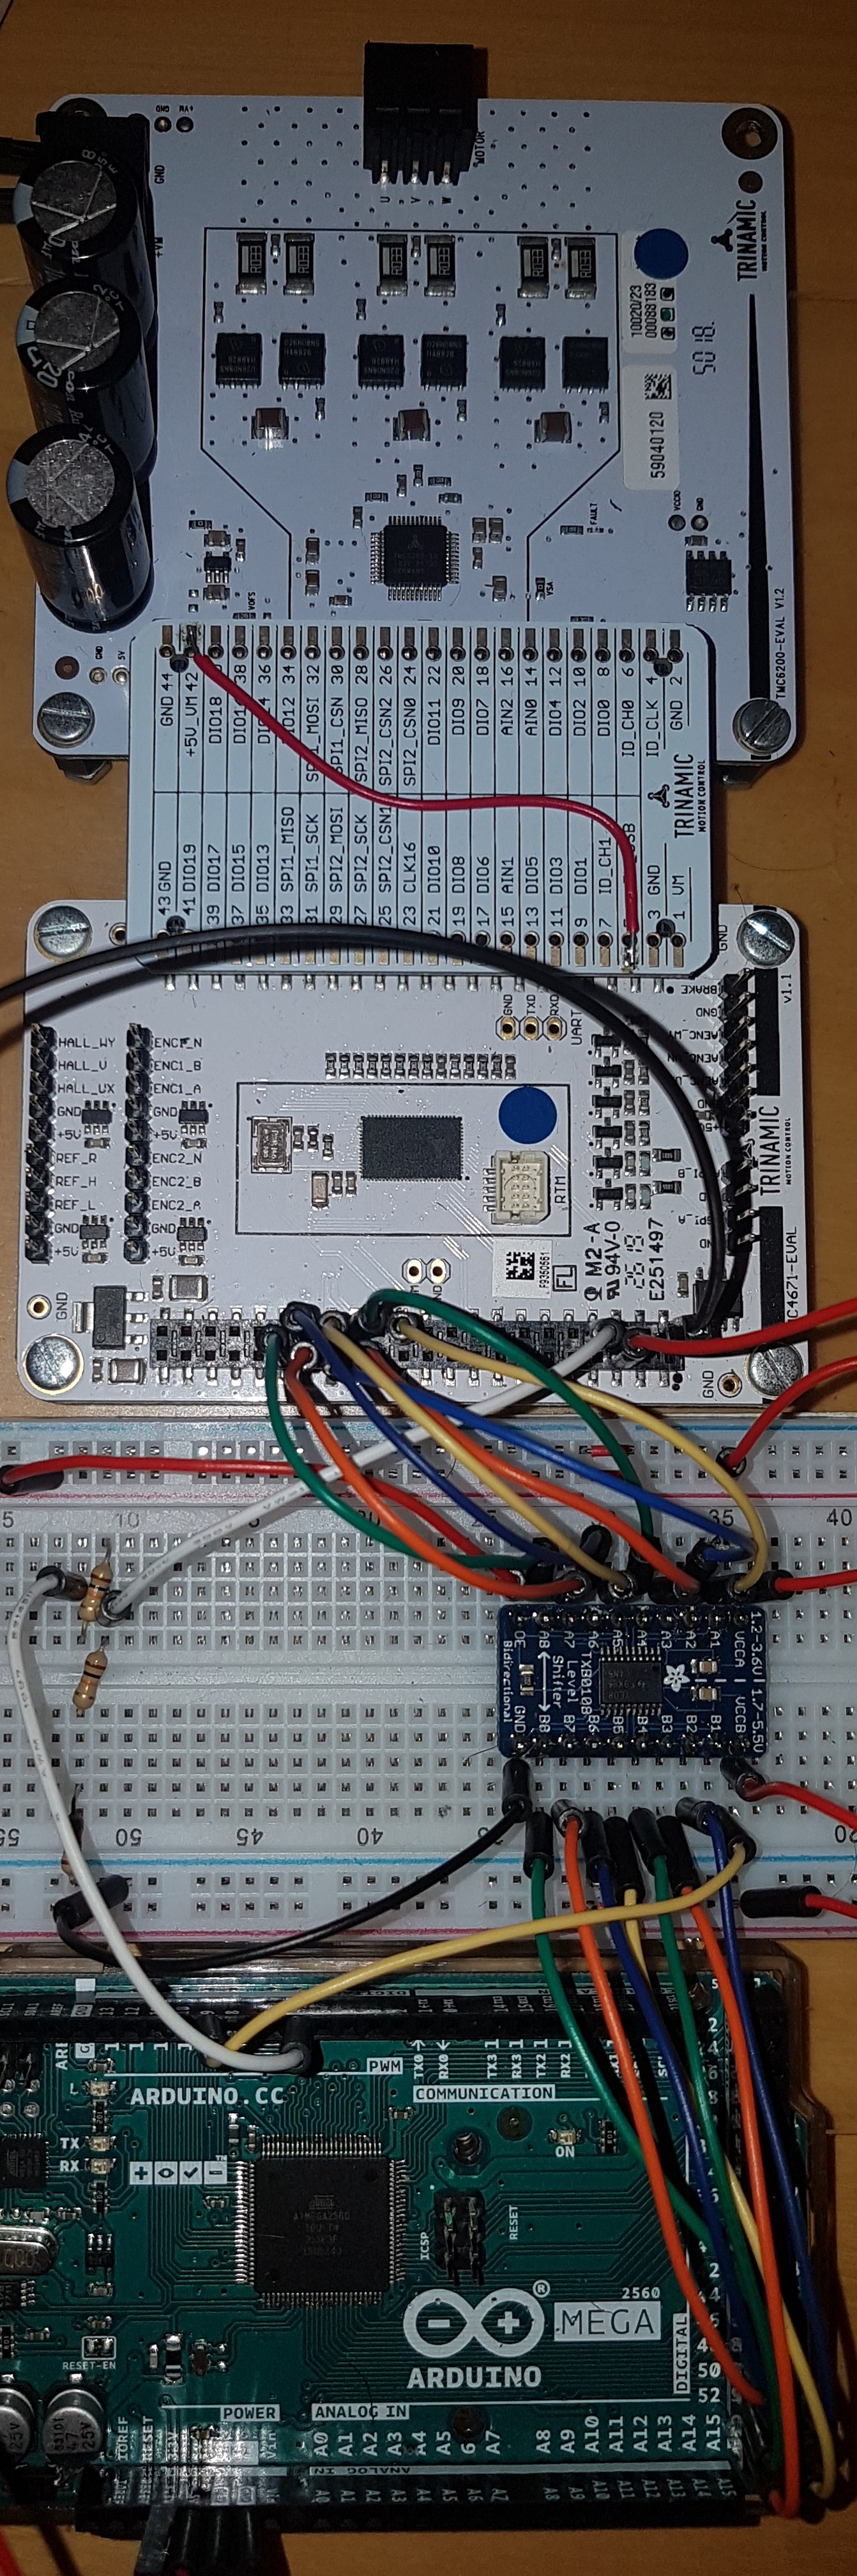
\includegraphics[angle=270,width=\textwidth]{graphics/2_komplett1}
	\caption{Gesamtansicht Setup.}
	\label{fig:2_komplett1}
\end{figure}

\textbf{Achtung}, wenn die Scripts auf den Mikrocontroller des PartyMixers geladen werden ist darauf zu achten, dass die Achse des Motors frei beweglich ist und das Förderband nicht mit der Achse mitdreht, da ansonsten Schäden an der Maschine entstehen können. Es wird empfohlen die Scripts mit Mikrocontroller und EVAL-Boards zu testen.

Vorgehen:
\begin{enumerate}
\item Benötigte Applikation, welche im Software-Ordner auf dem USB-Stick oder Github \cite{aebi_projekt-6softwareatmega_2020} zu finden ist, in Atmel Studio öffnen.\\
\textcolor{magenta}{Software\textrightarrow Atmega\textrightarrow 3\underline{ }Motor\underline{ }Openloop\textrightarrow 1\underline{ }Motor\underline{ }Testsoftware\textrightarrow Motor}\\


\item Software anpassen:\\
\textcolor{OliveGreen}{
	initTMC6200;\\
	initTMC4671\underline{ }Openloop();\\
\\
    while (1) \\
    \{\\
		\underline{ }delay\underline{ }ms(5000);\\
		read\underline{ }registers\underline{ }TMC6200();\\
		\underline{ }delay\underline{ }ms(10000);\\
		read\underline{ }registers\underline{ }TMC4671();\\
    \}
}\newline
\item Software hochladen:\\
\textcolor{blue}{AtmelStudio\textrightarrow Tools\textrightarrow PartyMixer}\\
\end{enumerate}

Ergebnis: Die Gate-CTRL-Signale liegen an und die H-Brücke schaltet den Leistungsteil, woran der Motor jetzt angeschlossen werden kann.

Im Anhang Kapitel \ref{Appendix:TMC6200_Gate_Ctrl} sind die aufbereiteten Gate-CTRL-Signale zu sehen und in Kapitel\ref{Appendix:H_Bruecke_Schaltsignale} die Messung der Schaltsignale.

Wird der Motor angeschlossen und der Mikrocontroller neu gestartet, der Motor sich mit der vorgegebenen Open-Loop-Geschwindigkeit.